\documentclass{article}
\usepackage[top=.5in, bottom=.5in, left=.9in, right=.9in]{geometry}
\usepackage[latin1]{inputenc}
\usepackage{enumerate}
\usepackage{hyperref}
\usepackage{graphics}
\usepackage{graphicx}
\usepackage{caption}
\usepackage{subcaption}
\usepackage{tabularx}
\usepackage{amsmath}
\usepackage{amssymb}
\usepackage{siunitx}
\usepackage{mathtools}

\newcommand{\obar}[1]{\ensuremath{\overline{ #1 }}}
\newcommand{\iid}{\ensuremath{\stackrel{\textrm{iid}}{\sim}}}

\usepackage{xcolor}
\definecolor{darkgreen}{rgb}{0,0.25,0}
\newcommand{\soln}{{\color{red}\textbf{Solution:~}\color{black}}}


\usepackage[formats]{listings}
\lstdefineformat{R}{~={\( \sim \)}}
\lstset{% general command to set parameter(s)
basicstyle=\small\ttfamily, % print whole listing small
keywordstyle=\bfseries\rmfamily,
keepspaces=true,
% underlined bold black keywords
commentstyle=\color{darkgreen}, % white comments
stringstyle=\ttfamily, % typewriter type for strings
showstringspaces=false,
numbers=left, numberstyle=\tiny, stepnumber=1, numbersep=5pt, %
frame=shadowbox,
rulesepcolor=\color{black},
,columns=fullflexible,format=R
} %
\renewcommand{\ttdefault}{cmtt}
% enumerate is numbered \begin{enumerate}[(I)] is cap roman in parens
% itemize is bulleted \begin{itemize}
% subfigures:
% \begin{subfigure}[b]{0.5\textwidth} \includegraphics{asdf.jpg} \caption{} \label{subfig:asdf} \end{subfigure}
\hypersetup{colorlinks=true, urlcolor=blue, linkcolor=blue, citecolor=red}


\graphicspath{ {C:/Users/Evan/Desktop/} }
\title{\vspace{-6ex}CSE 380: HW 0\vspace{-2ex}}
\author{Evan Ott \\ UT EID: eao466\vspace{-2ex}}
%\date{DATE}
\setcounter{section}{0}
\setcounter{subsection}{-1}
\setcounter{secnumdepth}{3}
\usepackage[parfill]{parskip}



\begin{document}
\maketitle
%0.0
\subsection{}
See Figures \ref{fig:country} and \ref{fig:segment} along with Tables \ref{tbl:country} and \ref{tbl:segment}.

The first
set of data could indicate plausibly one of two things: Italy and Saudi Arabia are competitive and want to have
the best supercomputers, or that there are (or were) features at the time in the country that make it easy to
build the best supercomputer (cheap electricity, increased funding, etc.).


\begin{figure}[h]
\begin{center}
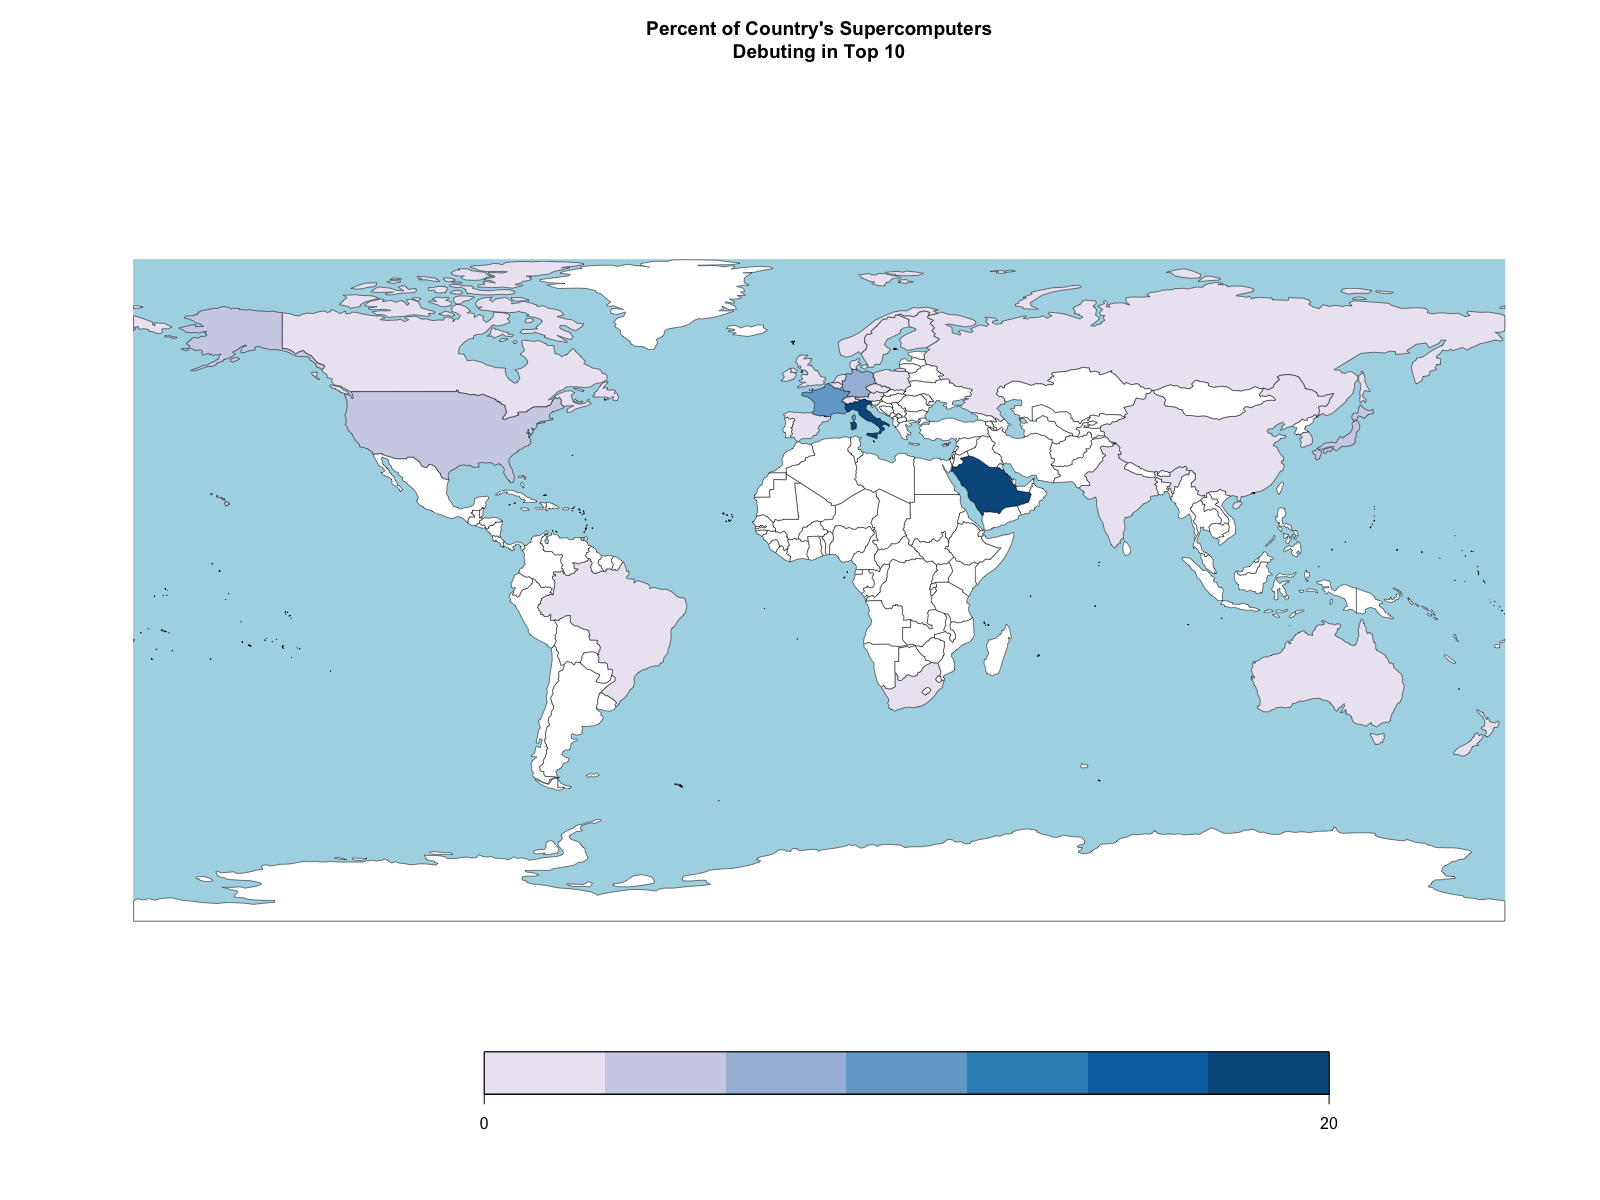
\includegraphics[scale=0.3]{country.png}
\caption{\label{fig:country}Percent of each country's supercomputers that debuted in the top 10.}
\end{center}
\end{figure}

% latex table generated in R 3.3.0 by xtable 1.8-2 package
% Fri Sep 30 16:24:00 2016
\begin{table}[ht]
\centering
\begin{tabular}{lr}
  \hline
Country & Value \\ 
  \hline
Italy & 20.00 \\ 
  Saudi Arabia & 20.00 \\ 
  France & 11.11 \\ 
  Germany & 7.69 \\ 
  United States & 5.45 \\ 
  Japan & 3.45 \\ 
  China & 2.38 \\ 
   \hline
\end{tabular}
\caption{\label{tbl:country}Percent of each country's supercomputers that debuted in the top 10. Countries on the top 500 that have not debuted in
the top 10: Australia, Austria, Belgium, Brazil, Canada, Czech Republic, Denmark, Finland, India, Ireland, Korea, South, Netherlands, New Zealand, Norway, Poland, Russia, Singapore, South Africa, Spain, Sweden, Switzerland, United Kingdom.}
\end{table}

The second set of data shows that in terms of applications, researchers and vendors may have a little bit more pride
in their supercomputer rankings than those in academia or general industry. Vendors have a major incentive to have
the best supercomputer (``look, our chips are the best!''), whereas academia doesn't (they just need it to work,
and will take what funding they can get from NSF to get things done). An interesting note here is that
there is only one on the list that is classified, and it debuted at rank 150. As for narrative with that one, it would
seem that governments doing classified work keep their supercomputers' specifications secret as to not reveal their
actual capabilities. So that's fun.

\begin{figure}[h]
\begin{center}
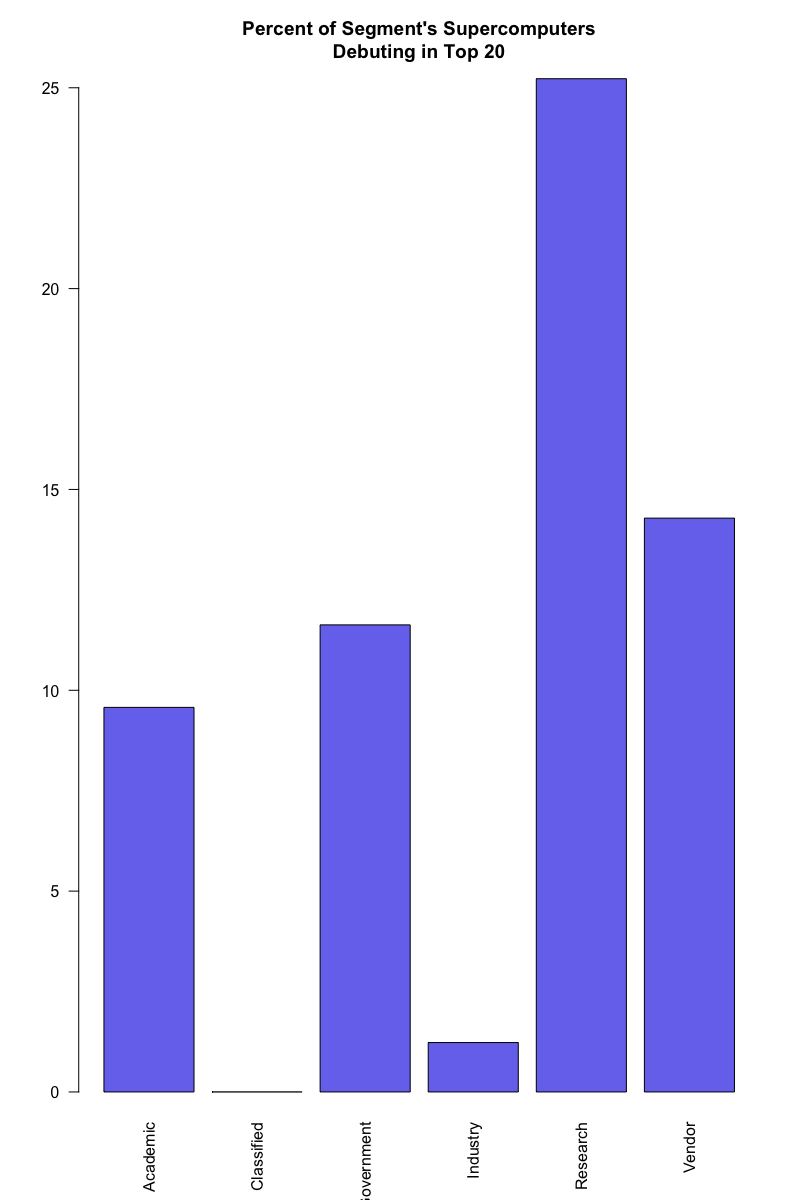
\includegraphics[scale=0.35]{barplot.png}
\caption{\label{fig:segment} Percent of segment's supercomputers debuting in top 20.}
\end{center}
\end{figure}

% latex table generated in R 3.3.0 by xtable 1.8-2 package
% Fri Sep 30 16:28:10 2016
\begin{table}[ht]
\centering
\begin{tabular}{lr}
  \hline
Segment & Value \\ 
  \hline
Research & 25.23 \\ 
  Vendor & 14.29 \\ 
  Government & 11.63 \\ 
  Academic & 9.57 \\ 
  Industry & 1.23 \\ 
  Classified & 0.00 \\ 
   \hline
\end{tabular}
\caption{\label{tbl:segment}Percent of segment's supercomputers debuting in top 20.}
\end{table}

\clearpage
\lstinputlisting[language=R]{hw0.R}

%0.1
\subsection{}
A Stampede core is ``faster'' than a Lonestar 4 core because it can do twice as many floating-point operations
per clock period. To show a full comparison:
\begin{table}[ht]
\begin{center}
\begin{tabular}{cccccc}
System & Clock Speed& flops / cp & Gflops / second & cores / node & Gflops / node\\
             & (GHz)          &                 &             (1 core)     &                     & (all cores)\\
\hline
Lonestar 4 &\textbf{3.33} & 4 & 13.32 & 12 & 159.84\\
Lonestar 5 & 2.6 & \textbf{8} & 20.8 & \textbf{24} & \textbf{499.2}\\
Stampede & 2.7 & \textbf{8} & \textbf{21.6} & 16 & 345.6
\end{tabular}
\end{center}
\end{table}

So in terms of floating-point operations per second (per core), Stampede is faster than Lonestar 5 is faster than Lonestar 4. However, in terms of peak performance per node, Lonestar 5 actually wins, followed by Stampede, then by Lonestar 4.
All this even though Lonestar 4 has the fastest clock speed.


%0.2
\subsection{}
\begin{itemize}
\item How many operations per clock cycle?
\begin{itemize}
	\item Intel Xeon E5-2680: 8 Flop / cp
\end{itemize}
\item Clock rate?
\begin{itemize}
	\item 2.7 GHz
\end{itemize}
\item 8 Flop / cp * 2.7 GHz = 21.6 GFlops
\item 8-way set associative L1 cache \cite{2680}. Assume 2 W / cp.
\begin{itemize}
	\item 2 * 2.7 * 8 = 43.2 GB/s
\end{itemize}
\item Assume $\sim$ 0.25 W/cp from main memory
\begin{itemize}
	\item 0.25 * 2.7 * 8 = 5.4 GB/s
\end{itemize}
\end{itemize}

%0.3
\subsection{}
\begin{verbatim}
# getent passwd | cut -f 7 -d: | sort | uniq
\end{verbatim}

The above command works as follows:
\begin{itemize}
\item bash reads the command, finding no splats or parts of the command that need to be filled in.
\item \texttt{getent} is called to query the Name Service Switch libraries to get the passwd database
\item \texttt{getent} returns (to standard output) a line for each user including username, group, name, home directory and shell, separated by colons.
\item The pipe redirects this standard output to standard input for \texttt{cut}, which takes the seventh field as separated by the ``:'' delimiter, which in the case of \texttt{getent passwd} is the location of the shell, and prints it to standard output.
\item The next pipe redirects to \texttt{sort}, which sorts the list alphanumerically. It outputs the same number of lines
as the input, but sorted.
\item The final pipe redirects to \texttt{uniq} which merges adjacent matching lines. As such, since the lines are already
sorted and all the matching lines will be next to each other, \texttt{uniq} will output each shell used on stampede
exactly once.
\end{itemize}


% 0.4
\subsection{}
\begin{verbatim}
# getent passwd | cut -f 7 -d: | sort | uniq --count | sort -bgr
  11504 /bin_bash
   8949 /bin/bash
    136 /bin_tcsh
     80 /bin/tcsh
     31 /sbin/nologin
     22 /bin/csh
     20 /bin_csh
     18 /bin/zsh
     13 /bin_zsh
      1 /sbin/shutdown
      1 /sbin/halt
      1 /bin/sync
\end{verbatim}
So 8948 active users on Stampede use bash, 80 use tcsh and the next most popular actual shell is csh.

%0.5
\subsection{}
\begin{verbatim}
# getent passwd | cut -f 1 -d: | awk '{print length(), $0}' | sort -g | tail -n1
13 avahi-autoipd
\end{verbatim}
avahi-autoipd is the longest TACC username, at 13 characters. It's the Avahi IPv4LL Stack
(from \texttt{finger avahi-autoipd}), so it's a user, just not necessarily a person. 

\begin{verbatim}
# getent passwd | cut -f 1 -d: | awk '{print length()}' | grep "8" | wc -l
10051
\end{verbatim}
10051 users have an 8-character username.


%0.6
\subsection{}
Question: How many usernames are a person's full name (first and last words in their name)?
\begin{verbatim}
# getent passwd | cut -f 1,5 -d: --output-delimiter " " | awk '{split($0, a, " "); \
username=a[1]; name = substr(tolower(sprintf("%s%s", a[2], a[length(a)])), 1, 8);\
f1 = index(username, name); f2 = index(name, username); print((f1 == f2) && (f1 == 1))}'\
| grep 1 | wc -l
766
\end{verbatim}



%0.7
\subsection{}
\subsubsection{}
\begin{verbatim}
# cat words | grep "^[a-zA-Z]" | awk '{print tolower(substr($0, 0, 1))}' | \
uniq --count | sed 's/ //g' | \
awk '{print substr($0, length($0), length($0)) ":" substr($0, 0, length($0) - 1)}'
a:31788
b:25192
c:40042
d:23263
e:17149
f:16263
g:15075
h:19317
i:15377
j:4426
k:6490
l:14680
m:26175
n:16668
o:15274
p:42073
q:3274
r:21688
s:51774
t:25875
u:23930
v:7019
w:12023
x:631
y:1820
z:1914
\end{verbatim}


\subsubsection{}
\begin{verbatim}
# cat words | awk '{print tolower($0)}' | grep "s$" | wc -l
86041
# cat words | awk '{print tolower($0)}' | grep "'s$" | wc -l
0
\end{verbatim}
The dictionary has 86,041 words that end in ``s'' but zero that are possessive (ends in ``'s'')

\subsubsection{}
\begin{verbatim}
# cat words | awk '{print tolower($0)}' | grep "foo[^dlt]\|foo$" | wc -l
37
\end{verbatim}
There are 37 words that contain the substring ``foo'' but not ``food'', ``fool'' or ``foot''. In other words,
the words contain ``foo'' followed by any character other than ``d'', ``l'', or ``t'' or ``foo'' must be the end of the string.


\subsubsection{}
Question: How many prefixes are there in the dictionary? Suffixes? What words have at least 4 dashes in them that aren't contiguous that aren't suffixes nor prefixes (i.e., cannot start nor end with a dash and have non-dashes in-between all dashes)?
\begin{verbatim}
# cat words | grep "\-$" | wc -l
1824
# cat words | grep "^-" | wc -l
560
# cat words | grep "[^-]\{1,\}-[^-]\{1,\}-[^-]\{1,\}-[^-]\{1,\}-[^-]\{1,\}" 
Jack-go-to-bed-at-noon
knock-down-and-drag-out
Mentor-on-the-Lake-Village
what-do-you-call-it
what-you-may-call-'em
\end{verbatim}

Related, looking at the 3-dash version of the above yields some great words such as ``king-of-the-salmon'' (a particular fish), ``stick-to-it-iveness'' (didn't know it was a proper word), ``toad-in-the-hole'' (British dish) and ``wag-on-the-wall'' (wall clock with elements exposed). I dunno, I thought these were esoteric enough to bring up as things more people should know.

I can't stop myself. What's the longest prefix? Longest suffix?
\begin{verbatim}
# cat words | grep "\-$" | awk '{print length, $0}' | sort -n| tail -n1
13 philosophico-
# cat words | grep "^-" | awk '{print length, $0}' | sort -n| tail -n1
10 -morphosis
\end{verbatim}

%0.8
\subsection{}
There is storage on each login node (\texttt{/tmp}), but ideally most or all data and work should be done
in one of the following three filesystems. \texttt{/tmp} is really for local I/O only, and usually \texttt{\$SCRATCH} should
be used in most cases instead.

\texttt{\$HOME} is permanent, has a quota and is backed up. It's used for storing code, executibles, things of that nature.

\texttt{\$WORK} is permanent, has a quota, but not backed-up. Code can be run here, and large files can be stored here.

\texttt{\$SCRATCH} is high-speed purged storage. It's a temporary workspace. Code can be run here, and large files can be stored here.

All three are Lustre parallel filesystems on 72 Dell R610 data servers through InfiniBand with four Dell R710 meta data servers and two Dell MD 3220 Storage Arrays. As stated on the TACC website, ``the interconnect is an FDR InfiniBand network of Mellanox switches, consisting of a fat tree topology of eight core-switches and over 320 leaf switches with a 5/4 oversubscription.''

There's also \texttt{\$ARCHIVE} which is tape storage through Ranch.

%0.9
\setcounter{subsection}{9}
\subsubsection{}
\begin{verbatim}
# uname -r
2.6.32-431.17.1.el6.x86_64
\end{verbatim}
The version is 2.6.32

\subsubsection{}
\begin{verbatim}
# curl https://www.kernel.org/pub/linux/kernel/v2.6/linux-2.6.32.27.tar.gz > \
linux-2.6.32.27.tar.gz && gunzip linux-2.6.32.27.tar.gz && tar -xvf linux-2.6.32.27.tar
\end{verbatim}
(I like seeing all the files as it unarchives them).

\subsubsection{}
\begin{verbatim}
# du -hc | tail -n1
418M	total
# find . | wc -l
   32365
# find . | grep '\.c$' | wc -l
   13149
\end{verbatim}
This version of Linux is 418 megabytes. Including directories (everything is a file or process!), this version has 32365 files, 13149 of which are .c files.

\subsubsection{}
\begin{verbatim}
# ls -R | grep "^\..*:$" | wc -l
1878
# find . -type d | wc -l
1878
# tree -d -i --noreport | wc -l
1878
\end{verbatim}

\subsubsection{}
\begin{verbatim}
# find . | grep '\.[hc]$' | xargs wc -l | sort -bg | grep "\.[hc]$" | tail -n1
   17722 ./sound/pci/hda/patch_realtek.c
\end{verbatim}
The /sound/pci/hda/patch\_realtek.c file is the largest (in terms of lines of code) and has 17,722 lines.

\subsubsection{}
\begin{verbatim}
# find . | grep '\.[hc]$' | xargs wc -l | tail -n1
 828952 total
\end{verbatim}
Including comments, there are 828,952 lines of code in this version of the Linux kernel.

\subsubsection{}
Question: How many \texttt{main} functions are there? How many versions have the canonical argument names \texttt{int argc} and \texttt{char *argv}?

\begin{verbatim}
# find . | grep '\.[hc]$' | xargs grep "int main(int .*, char .*)"
   51
# find . | grep '\.[hc]$' | xargs grep "int main(int argc, char \*argv\[\])" | wc -l
   27
\end{verbatim}

\begin{thebibliography}{9}
\bibitem{2680} \url{http://www.cpu-world.com/CPUs/Xeon/Intel-Xeon%20E5-2680.html}
\end{thebibliography}
\end{document}